\documentclass[20pt]{beamer}
\input{preambulemanu.sty}
\usetheme{CambridgeUS}    % theme rouge
\title[Fonctions polynômes]{Cours}
\author{E.~COZIC}
\date{\today}
% -----------------

\begin{document}

\begin{frame}          % Transparent 1
  \titlepage
\end{frame}



%%%%%%%%%%%%%%%%%%%%%%%%%%%%%%%%%%%%%%%%%%%%%%%

\begin{frame}          % Transparent 2
\begin{center}
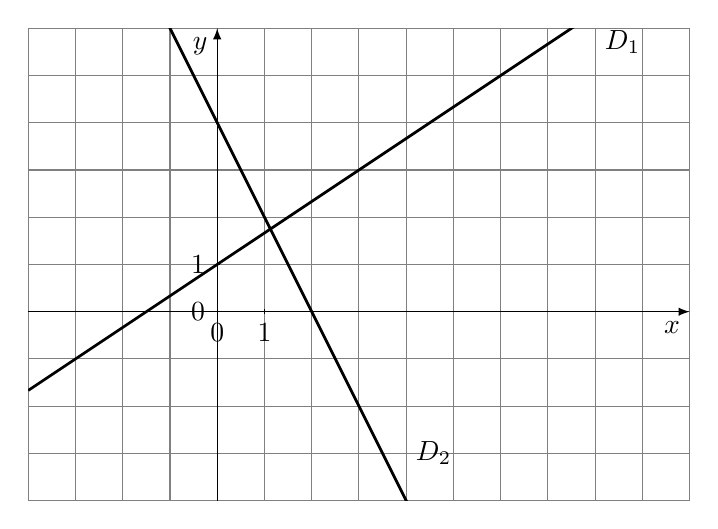
\begin{tikzpicture}[scale=0.6]

\draw [gray,xstep=1,ystep=1] (-4,-4) grid (10,6);
\draw [->,>=latex] (-4,0) -- (10,0) node [below left] {$x$};
\draw [->,>=latex] (0,-4) -- (0,6) node [below left] {$y$};

\foreach \x in {0,...,1}
\draw (\x,0.5mm) -- (\x,-0.5mm) node [below] {$\x$};
\foreach \y in {0,...,1}
\draw (0.5mm,\y) -- (-0.5mm,\y) node [left] {$\y$};

\clip (-4,-4) rectangle (10,6);
\draw [domain=-4:10,line width=1pt,samples=100] plot (\x,{2/3*\x+1});
\draw [domain=-4:10,line width=1pt,samples=100] plot (\x,{-2*\x+4});


\draw (8,5.7) node [right] {$\mathscr{D}_{1}$};
\draw (4,-3) node [right] {$\mathscr{D}_{2}$};

\end{tikzpicture}
\end{center}
\end{frame}
%%%%%%%%%%%%%%%%%%%%%%%%%%%%%%%%%%%%%%%%%%%%%%%
\begin{frame}          % Transparent 3

\begin{center}
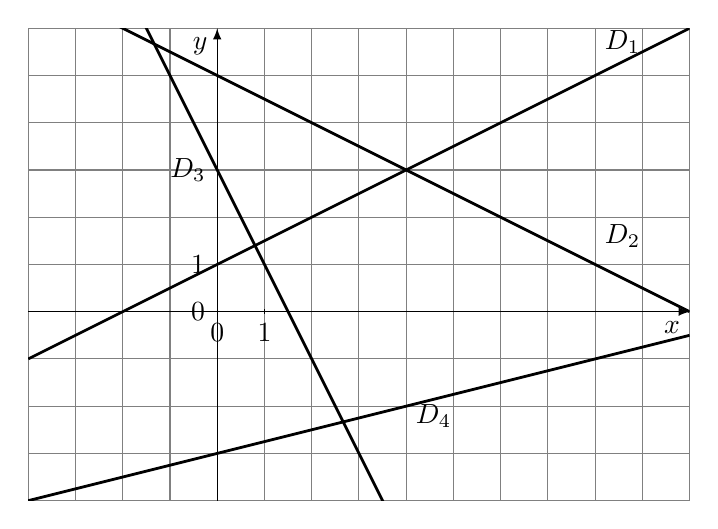
\begin{tikzpicture}[scale=0.6]

\draw [gray,xstep=1,ystep=1] (-4,-4) grid (10,6);
\draw [->,>=latex] (-4,0) -- (10,0) node [below left] {$x$};
\draw [->,>=latex] (0,-4) -- (0,6) node [below left] {$y$};

\foreach \x in {0,...,1}
\draw (\x,0.5mm) -- (\x,-0.5mm) node [below] {$\x$};
\foreach \y in {0,...,1}
\draw (0.5mm,\y) -- (-0.5mm,\y) node [left] {$\y$};

\clip (-4,-4) rectangle (10,6);
\draw [domain=-4:10,line width=1pt,samples=100] plot (\x,{(-2)*\x+3});
\draw [domain=-4:10,line width=1pt,samples=100] plot (\x,{1/2)*\x+1});
\draw [domain=-4:10,line width=1pt,samples=100] plot (\x,{(-1/2)*\x+5});
\draw [domain=-4:10,line width=1pt,samples=100] plot (\x,{(1/4)*\x-3});

\draw (8,5.7) node [right] {$\mathscr{D}_{1}$};
\draw (8,1.6) node [right] {$\mathscr{D}_{2}$};
\draw (-1.2,3) node [right] {$\mathscr{D}_{3}$};
\draw (4,-2.2) node [right] {$\mathscr{D}_{4}$};
\end{tikzpicture}
\end{center}
\end{frame}

%%%%%%%%%%%%%%%%%%%%%%%%%%%%%%%%%%%%%%%%%%%%%%%

\begin{frame}          % Transparent 4
\begin{center}
\begin{tikzpicture}[scale=1.5]
\tkzInit[xmin=-3,xmax=3,ymin=-1,ymax=3]
\draw [->] (-3,0) -- (3,0) node [below right] {$x$};
\draw [->] (0,-1) -- (0,3) node [below right] {$y$}; 

\draw[domain= -1.2:1.2]
                plot (\x, {2*(\x)^2)} );
\draw[line width=1pt, color=red,domain = -1.2:1.2]
                plot (\x, {2*(\x)^2)+1} ); 
\draw[line width=1pt,color=red,->] (0,0) --(0,1);
\draw (1,1) node[right]{$f(x)=2x$};
\draw (1,3.2) node[color=red,right]{$f(x)=2x+1$};
\draw (0.1,0.5) node[color=red,left]{$\vv{j}$};
\draw (0,1) node {$\bullet$}; 
\draw (0.2,1.1) node[color=blue,above]{$S$};
\end{tikzpicture}
\end{center}
\end{frame}

\begin{frame}          % Transparent 5
\begin{center}
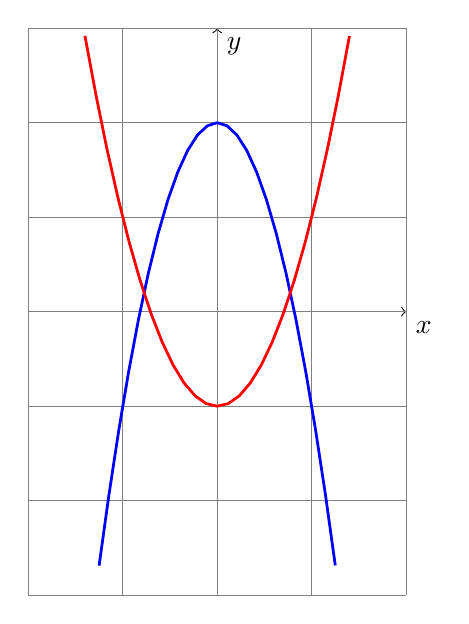
\begin{tikzpicture}[scale=1.2]
\tkzInit[xmin=-2,xmax=2,ymin=-3,ymax=3]
\tkzInit[xmin=-2,xmax=4,ymin=-1,ymax=5]
\draw [->] (-2,0) -- (2,0) node [below right] {$x$};
\draw [->] (0,-3) -- (0,3) node [below right] {$y$};
\draw[gray](-2,-3) grid(2,3);
\draw[color=blue,line width=1pt, domain=-1.25:1.25]
                plot (\x, {-3*(\x)^2+2)} );
\draw[line width=1pt, color=red,domain = -1.4:1.4]
                plot (\x, {2*(\x)^2)-1} ); 

\draw (-1,-1) node[color=blue,left]{$\Cf$};
\draw (1.2,2.2) node[color=red,right]{$\Cg$};

\end{tikzpicture}

\end{center}
\end{frame}


\begin{frame}          % Transparent 6
\begin{center}
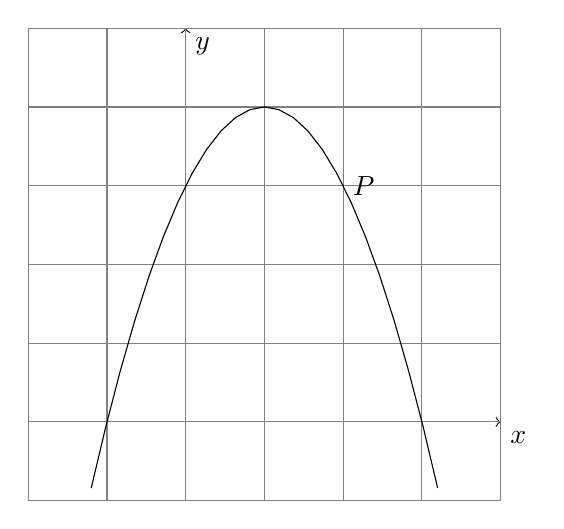
\begin{tikzpicture}[scale=1]
\tkzInit[xmin=-2,xmax=4,ymin=-1,ymax=5]
\draw [->] (-2,0) -- (4,0) node [below right] {$x$};
\draw [->] (0,-1) -- (0,5) node [below right] {$y$};
\draw[gray](-2,-1) grid(4,5);
\draw[domain=-1.2:3.2] plot (\x, {-1*(\x+1)*(\x-3)} ) ;
\draw (2,3) node[right]{$\mathscr{P}$};
\end{tikzpicture}



\end{center}
\end{frame}


\begin{frame}          % Transparent 7
\begin{center}
    

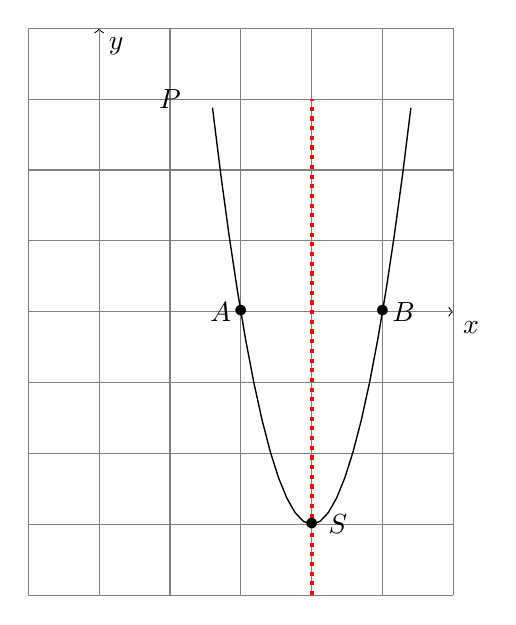
\begin{tikzpicture}[scale=0.9]
\tkzInit[xmin=-1,xmax=5,ymin=-4,ymax=4]
\draw [->] (-1,0) -- (5,0) node [below right] {$x$};
\draw [->] (0,-4) -- (0,4) node [below right] {$y$};
\draw[gray](-1,-4) grid(5,4);
\draw[line width=0.5pt,domain=1.6:4.4] plot (\x, {3*(\x-2)*(\x-4)} ) ;
\draw (1,3) node{$\mathscr{P}$};
\draw[line width=1.5pt,color=red,dotted] (3,-4)--(3,3);
\draw (3.1,-3) node[right]{$S$};
\draw (3,-3) node{$\bullet$};
\draw (2,0) node{$\bullet$};
\draw (4,0) node{$\bullet$};
\draw (2,0) node[left]{$A$};
\draw (4,0) node[right]{$B$};
\end{tikzpicture}
\end{center}
\end{frame}


\end{document}